\chapter{Komunikace s platformou}
\label{sec:PlatformCommunication}
\vspace{-20pt}
\

V této kapitole je popsán způsob zobrazení a ukládání dat během jízdy.

Během jízdy je důležité posílat data asynchronně, aby nebyl  blokován hlavní algoritmu auta.
Z toho důvodu pro komunikaci s platformou je použit \textbf{UDP}
(User Datagram Protocol) protokol. UDP je komunikační protokol,
který se primárně používá pro časově citlivé informace.
Zrychluje komunikaci tím, že před přenosem dat není nutné formálně navazovat spojení, což umožňuje velmi rychlý přenos dat\cite{UDP}.

Během komunikace se vývojová deska chová jako UDP server a klient
pro server je apliakce sloužící k zobrazení dat. Aplikace pro zobrazení dat jsem pojmenoval jako \textbf{CarQt}. CarQt umí zobrazovat: 
\begin{itemize}
    \item Originální obraz;
    \item Normalizovány obraz;
    \item Prahový obraz.
\end{itemize}

Další data jsou zobrazeny v číselném formátu. To je informace o:
\begin{itemize}
    \item Regiony;
    \item PWM motor;
    \item Servo motor;
    \item Senzory.
\end{itemize}
data z kamery ve 2D formátu s~historii záznamu. Zobrazuje originální, normalizovány a prahový obraz. Další data
jsou zobrazeny v číselném formátu. To jsou informace o regionu, PWM motoru, servo motoru
a senzoru. Ukládání číselných dat je implementováno ve formátu \textbf{JSON}
(JavaScript Object Notation) a originálního obrazu ve formátu \textbf{PNG}
(Portable Network Graphics) souboru. CarQt je napsána pomocí knihoven Qt a OpenCV.
Aplikace je zobrazena na obrázku \ref{fig:CarQt}
\begin{figure}[!h]
    \centering
    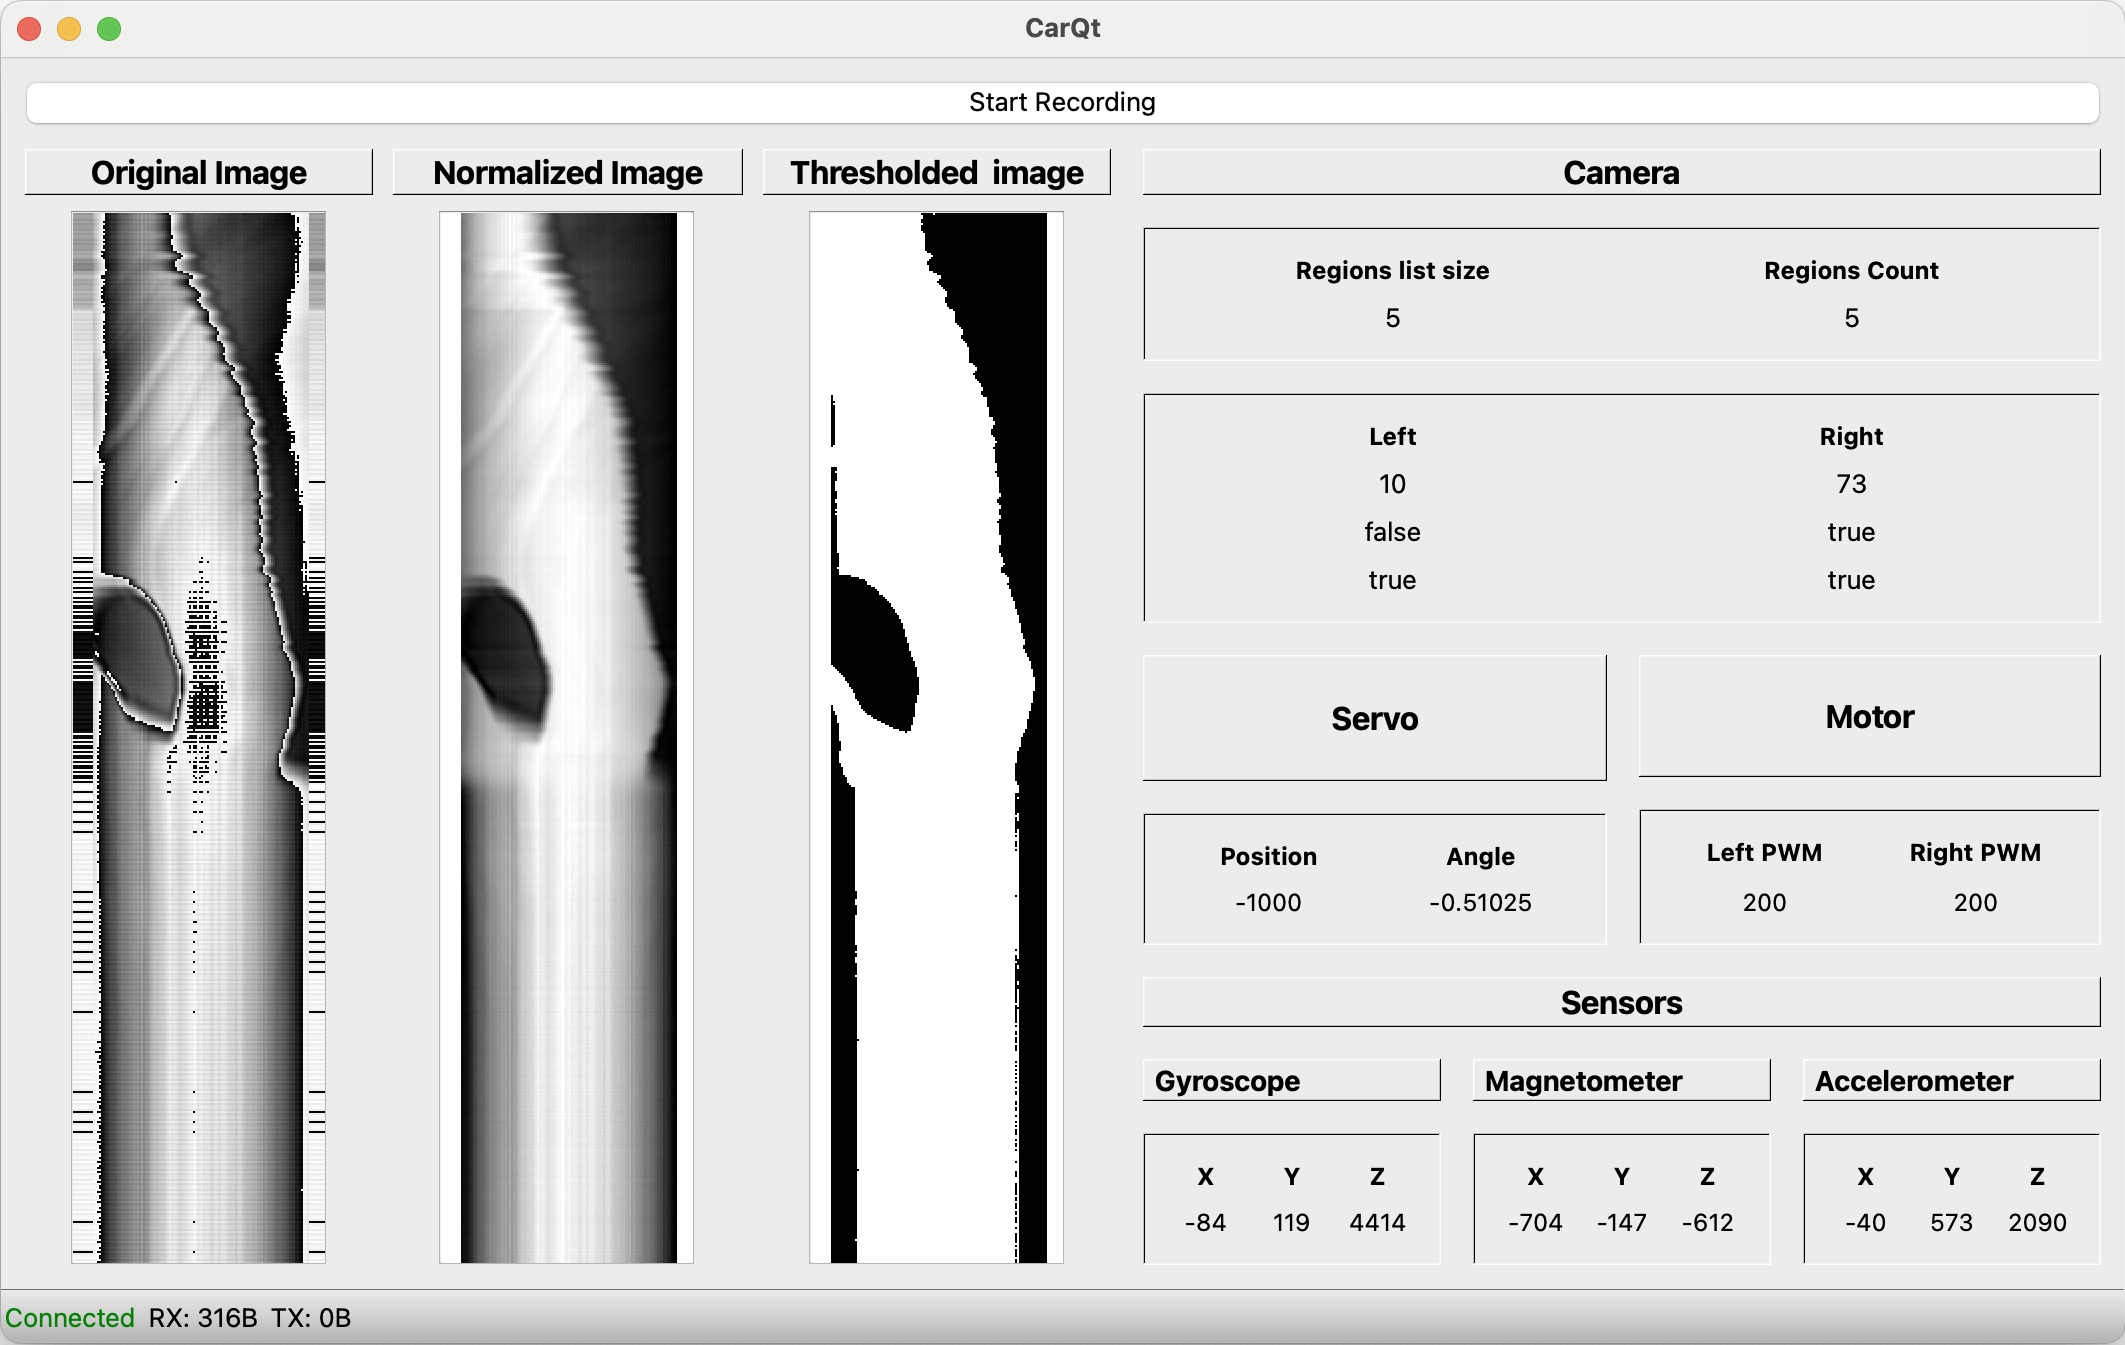
\includegraphics[width = .5\linewidth]{Figures/CarQt.png}
    \caption{CarQt aplikace}
    \label{fig:CarQt}
\end{figure}


Pro přenos a ukládání dat je použita struktura \textbf{Data}, která obsahuje originální data z kamery, Regionu, PWM motoru, servo motoru a senzoru. Implementovaná struktura Data je ve výpisu \ref{lst:data}
\begin{lstlisting}[caption=structura Data, label=lst:data]
// Data.h
struct Data {
    // Camera data
    uint16_t line[Image::LINE_LENGTH] = {0};
    uint32_t regionsCount = 0;
    uint32_t regionsListSize = 0;
    bool unchangedLeft = false;
    bool unchangedRight = false;
    bool hasLeft = false;
    bool hasRight = false;
    uint8_t leftDistance = 0;
    uint8_t rightDistance = 0;

    // Motor data
    int32_t leftSpeed = 0;
    int32_t rightSpeed = 0;

    // Servo data
    int32_t servoPosition = 0;
    float angle = .0f;

    Vec3<int16_t> accel = {0, 0, 0};
    Vec3<int16_t> mag = {0, 0, 0};
    Vec3<int16_t> gyro = {0, 0, 0};

    uint32_t timestamp = 0;
    uint8_t mode = Mode::None;
};
\end{lstlisting}

\endinput
